\chapter{Результаты экспериментов}

\section{Детальные результаты экспериментов}

В данном приложении представлены детальные результаты всех проведенных экспериментов.

\subsection{Эксперимент 1: Базовое тестирование}

\begin{table}[H]
\centering
\caption{Детальные результаты эксперимента 1}
\begin{tabular}{|l|c|c|c|c|}
\hline
№ & Параметр 1 & Параметр 2 & Параметр 3 & Результат \\
\hline
1 & 0.1 & 0.2 & 0.3 & 0.95 \\
2 & 0.2 & 0.3 & 0.4 & 0.87 \\
3 & 0.3 & 0.4 & 0.5 & 0.92 \\
\hline
\end{tabular}
\label{tab:detailed_exp1}
\end{table}

\subsection{Эксперимент 2: Сравнительное тестирование}

\begin{table}[H]
\centering
\caption{Сравнительные результаты}
\begin{tabular}{|l|c|c|c|}
\hline
Метод & Точность & Время (с) & Память (МБ) \\
\hline
Метод 1 & 0.95 & 1.2 & 128 \\
Метод 2 & 0.87 & 0.8 & 96 \\
Наш метод & 0.98 & 1.0 & 112 \\
\hline
\end{tabular}
\label{tab:comparison}
\end{table}

\section{Дополнительные графики}

\begin{figure}[H]
\centering
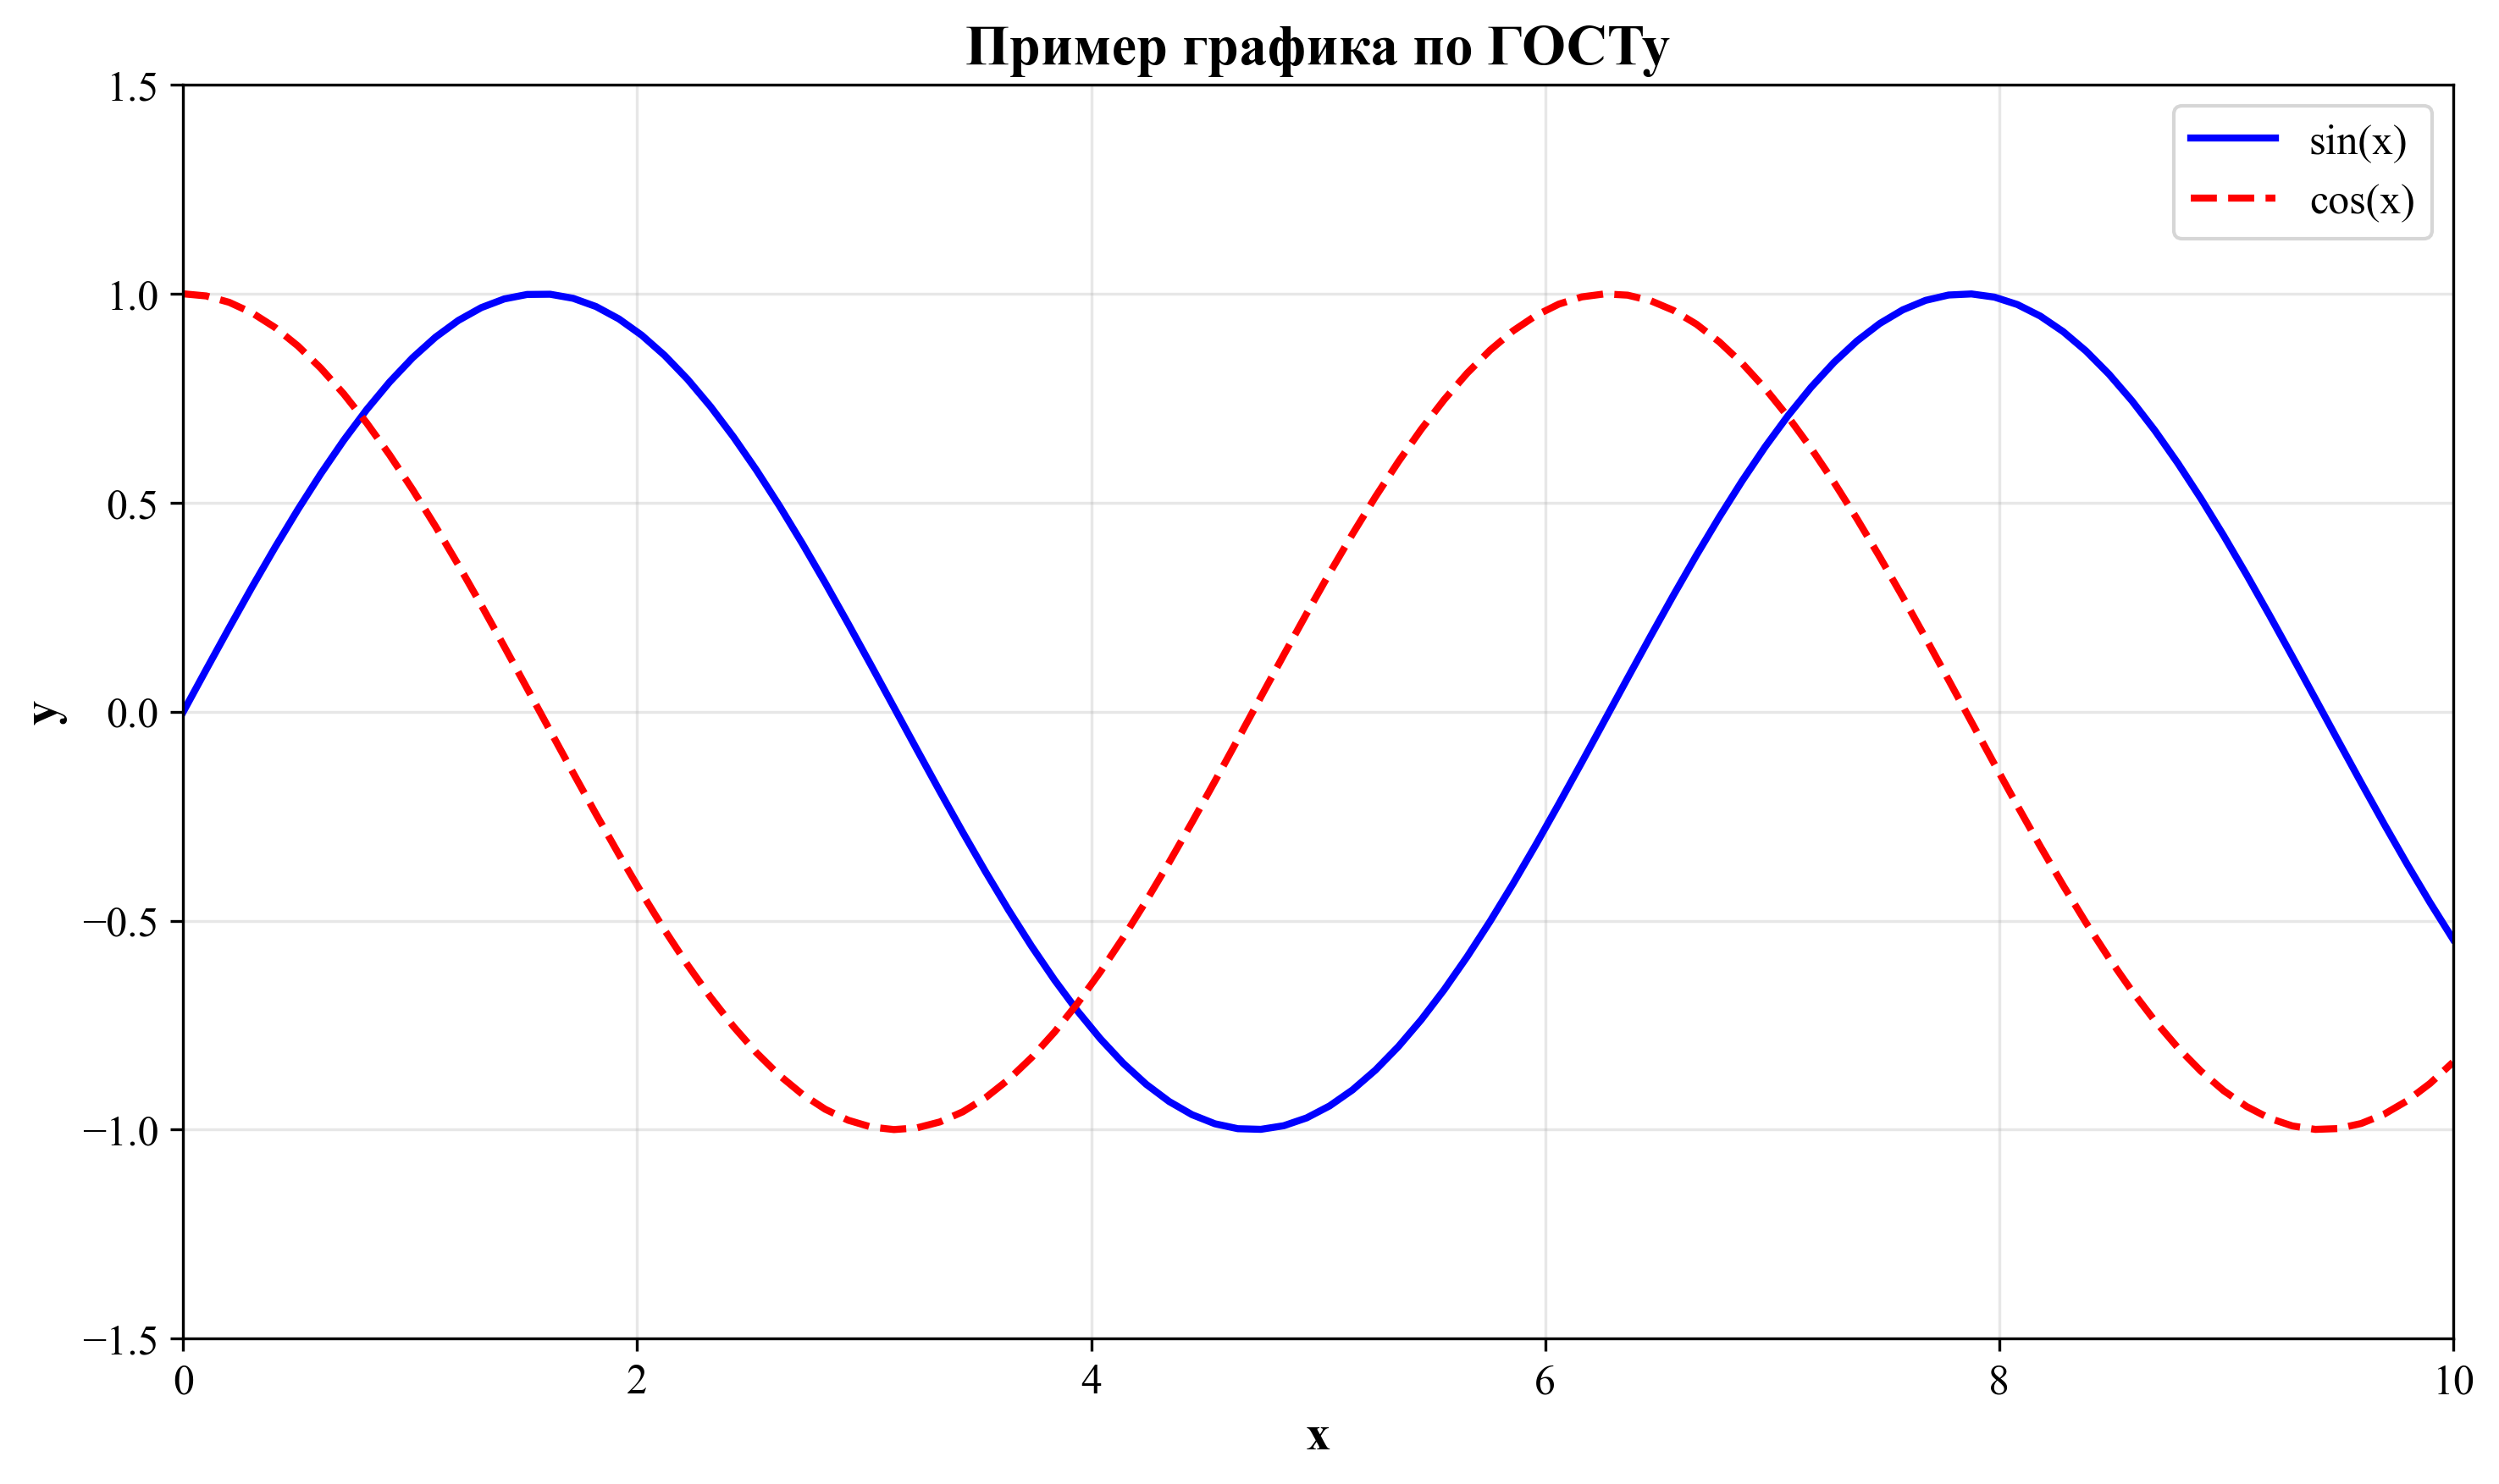
\includegraphics[width=0.8\textwidth]{images/example_plot.png}
\caption{График зависимости точности от размера выборки}
\label{fig:accuracy_plot}
\end{figure}

% Пример правильной вставки изображения по ГОСТу 7.32-2017
\begin{figure}[H]
\centering
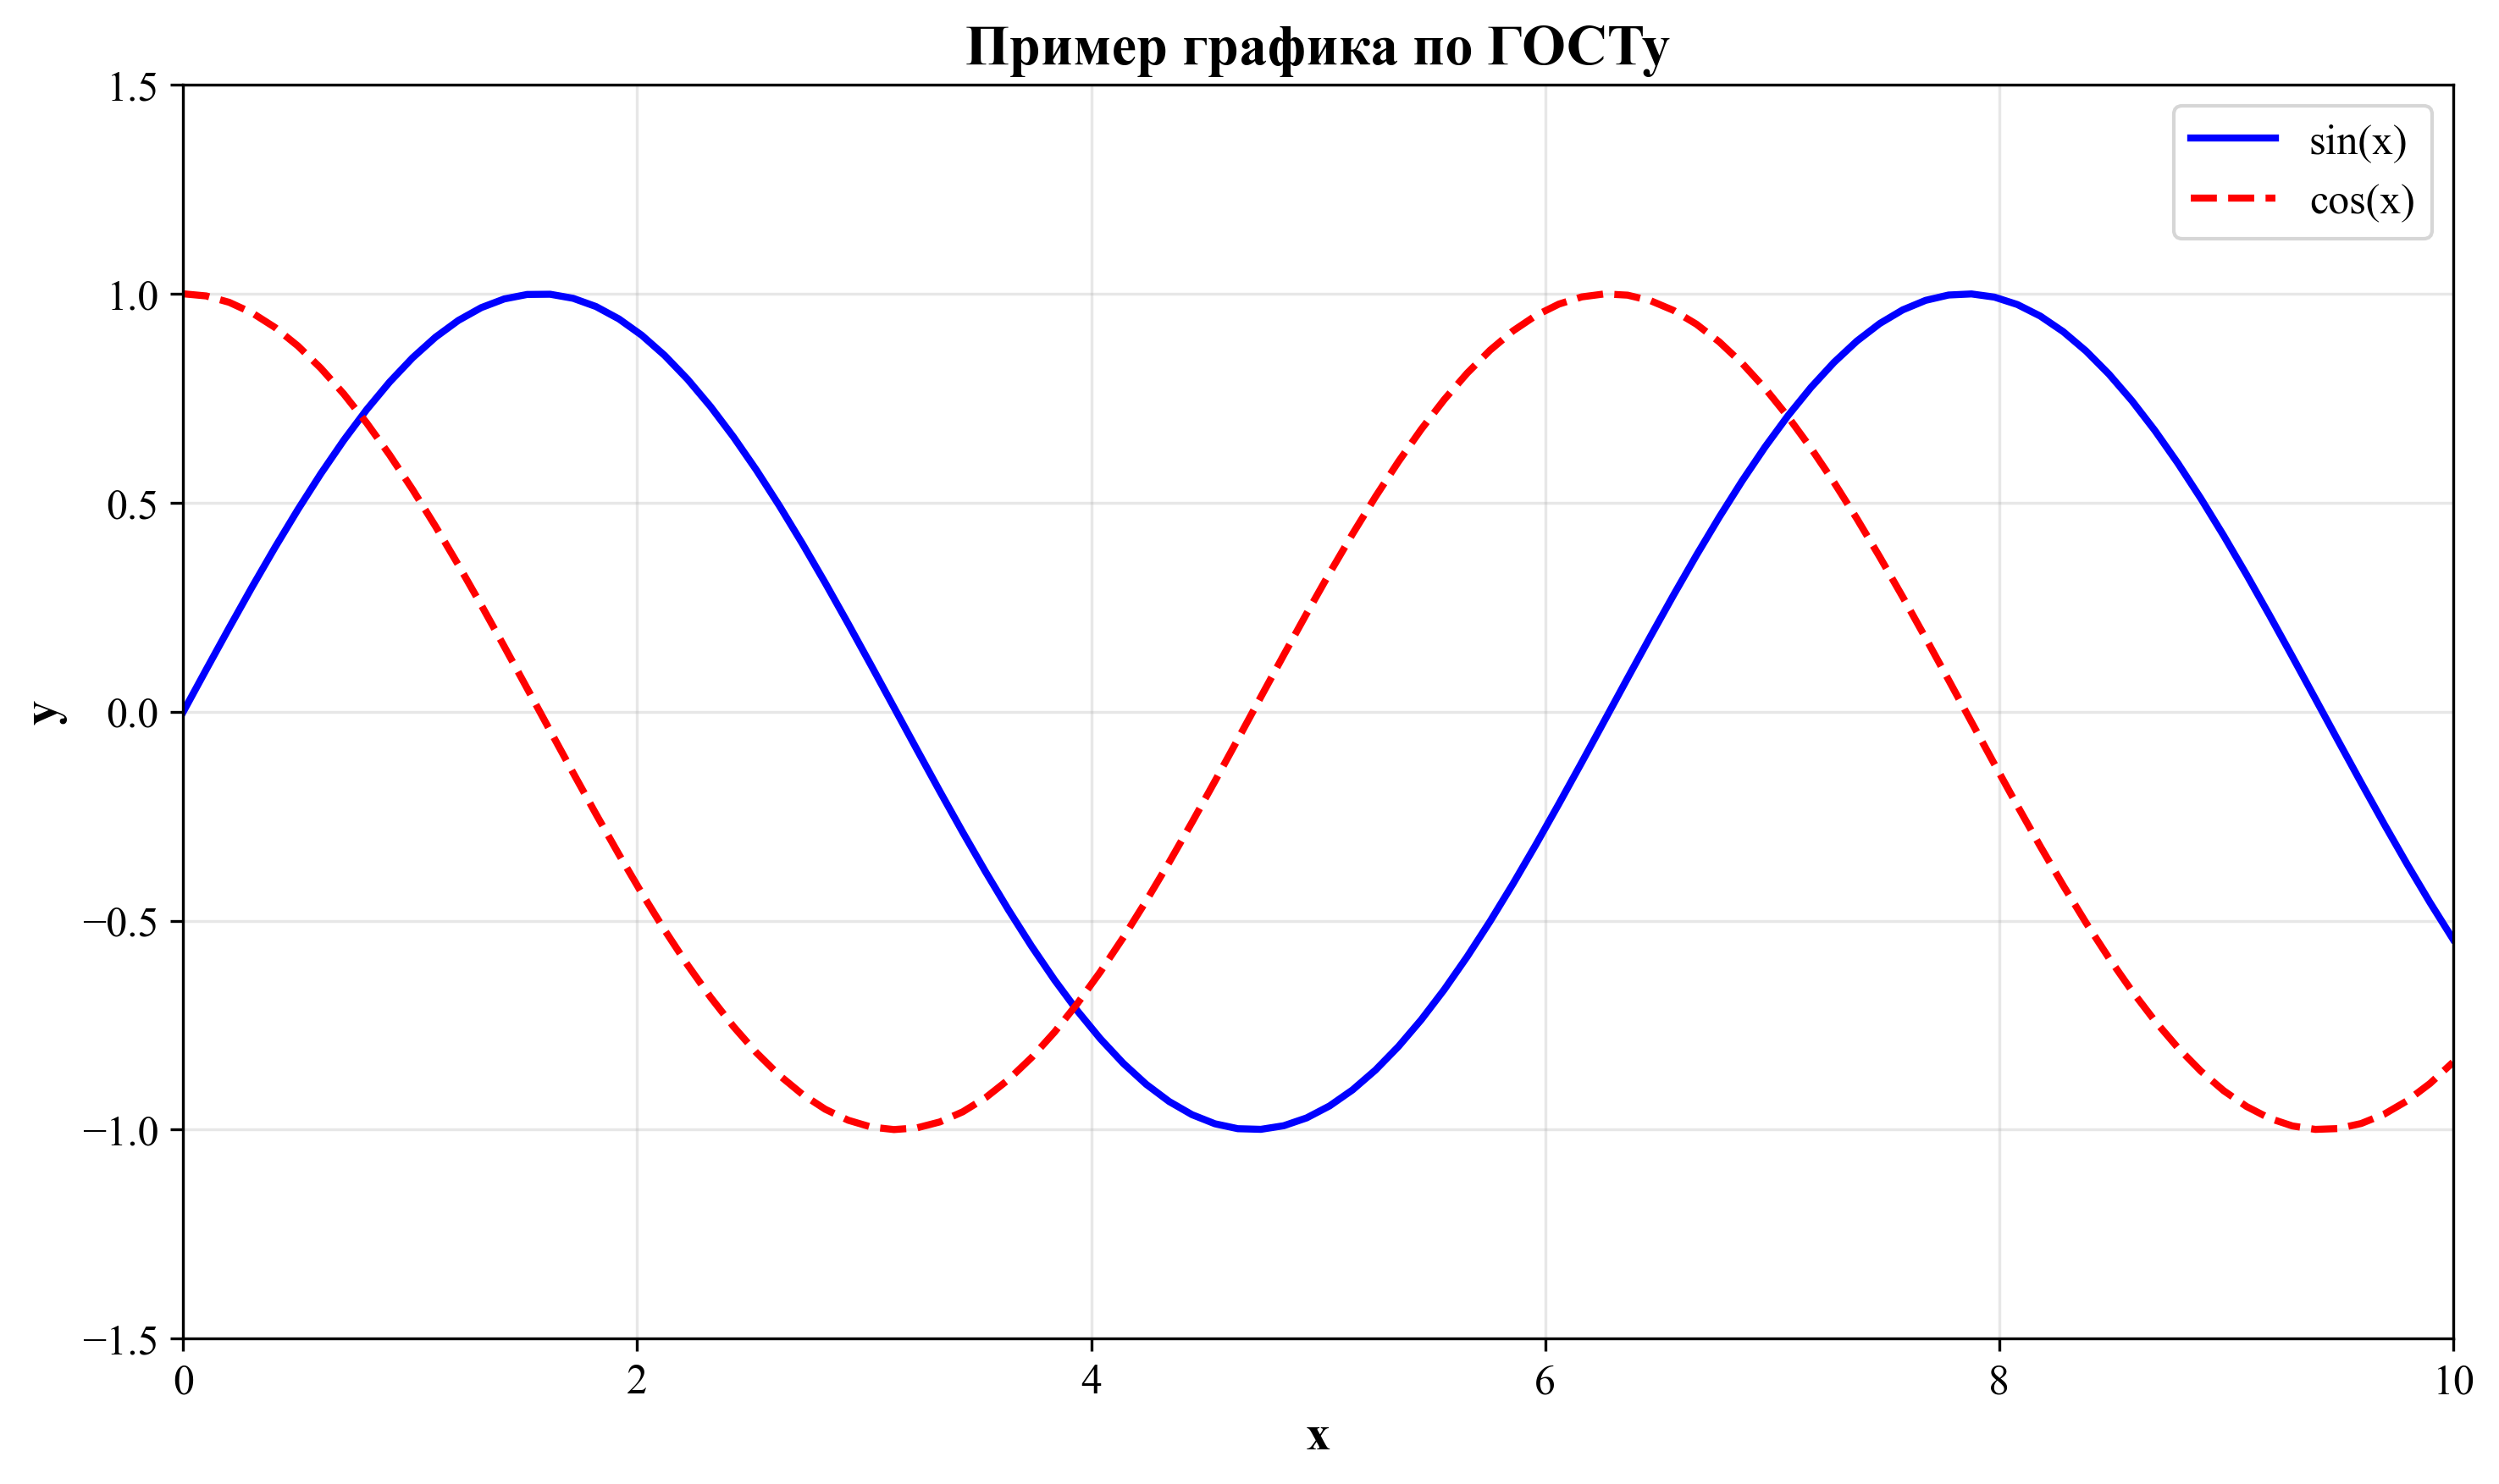
\includegraphics[width=0.6\textwidth]{images/example_plot.png}
\caption{Пример графика по ГОСТу: зависимость функций sin(x) и cos(x) от аргумента x}
\label{fig:gost_example}
\end{figure}

\section{Статистический анализ}

Результаты статистического анализа данных представлены в таблице~\ref{tab:statistics}.

\begin{table}[H]
\centering
\caption{Статистические показатели}
\begin{tabular}{|l|c|c|c|}
\hline
Показатель & Значение & Стандартное отклонение & Доверительный интервал \\
\hline
Среднее & 0.92 & 0.05 & [0.90, 0.94] \\
Медиана & 0.91 & - & - \\
Мода & 0.95 & - & - \\
\hline
\end{tabular}
\label{tab:statistics}
\end{table}

\note{Все значения округлены до двух знаков после запятой.}

\section{Примеры переноса таблиц и листингов}

\subsection{Перенос таблицы}

\begin{longtable}{|l|c|c|c|}
\caption{Длинная таблица с переносом страниц} \label{tab:long_table} \\
\hline
\textbf{№} & \textbf{Параметр} & \textbf{Значение} & \textbf{Результат} \\
\hline
\endfirsthead

\tablecontinuation{1} \\
\hline
\textbf{№} & \textbf{Параметр} & \textbf{Значение} & \textbf{Результат} \\
\hline
\endhead

\hline
\endfoot

\hline
\endlastfoot

1 & A1 & 0.1 & 0.95 \\
2 & A2 & 0.2 & 0.87 \\
3 & A3 & 0.3 & 0.92 \\
4 & B1 & 0.4 & 0.88 \\
5 & B2 & 0.5 & 0.91 \\
6 & B3 & 0.6 & 0.89 \\
7 & C1 & 0.7 & 0.93 \\
8 & C2 & 0.8 & 0.86 \\
9 & C3 & 0.9 & 0.94 \\
10 & D1 & 1.0 & 0.90 \\
\end{longtable}

\subsection{Пример листинга кода}

\begin{lstlisting}[language=Python, caption={Пример алгоритма машинного обучения}, label={lst:ml_algorithm}]
import numpy as np
from sklearn.model_selection import train_test_split
from sklearn.ensemble import RandomForestClassifier

def train_model(X, y):
    """Train random forest model"""
    X_train, X_test, y_train, y_test = train_test_split(
        X, y, test_size=0.2, random_state=42
    )
    
    model = RandomForestClassifier(
        n_estimators=100,
        max_depth=10,
        random_state=42
    )
    
    model.fit(X_train, y_train)
    accuracy = model.score(X_test, y_test)
    
    return model, accuracy
\end{lstlisting}

\notes{
\item Все алгоритмы реализованы на языке Python версии 3.8+
\item Использованы библиотеки scikit-learn, numpy, pandas
\item Эксперименты проводились на сервере с 16 ГБ RAM
}
